\section{Self-supervised image restoration via THz SAHS images}
\subsection{Data Acquisition}
THz SAHS images were acquired using a THz-TDS reflection setup, as shown in Fig.~\ref{fig:system}. THz pulses were generated using femtosecond and photoconductive antennas. The femtosecond laser featured a central wavelength of 1.5 μm and a pulse width of 80 fs. A fiber-coupled antenna (TERA15-TX-FC, Menlo Systems) was used as the photoconductive antenna to generate THz pulses, and another fiber-coupled dipole antenna (TERA15-RX-FC, Menlo Systems) was used to detect THz signals. To acquire THz signals rapidly, we employed an ultrafast scanner with a frequency and time width of 20 Hz and 30ps, respectively.

The THz signal was amplified using a low-noise current preamplifier (SRS570, Stanford Research) and subsequently digitized using a data-acquisition board. The generated THz pulses were guided through polymethylpentene (TPX) lenses and plate mirrors. The TPX lens focused the THz signal onto the sample stage, and the signal reflected from the sample was guided to the detector through a silicon beam splitter andanother TPX lens. All components except for the sample were placed within a dry air chamber to avoid signal distortion due to water vapor absorption. To obtain a two-dimensional image, the sample was shifted along the x- and y-axes to form a THz image with a spatial resolution of 282$\times$282 pixels, totaling 79,524 pixels. The time-domain signals obtained at each pixel were transformed into the frequency domain via the fast Fourier transform (FFT) to acquire broadband THz-wave characteristics.

\begin{figure}[htbp]
    \centering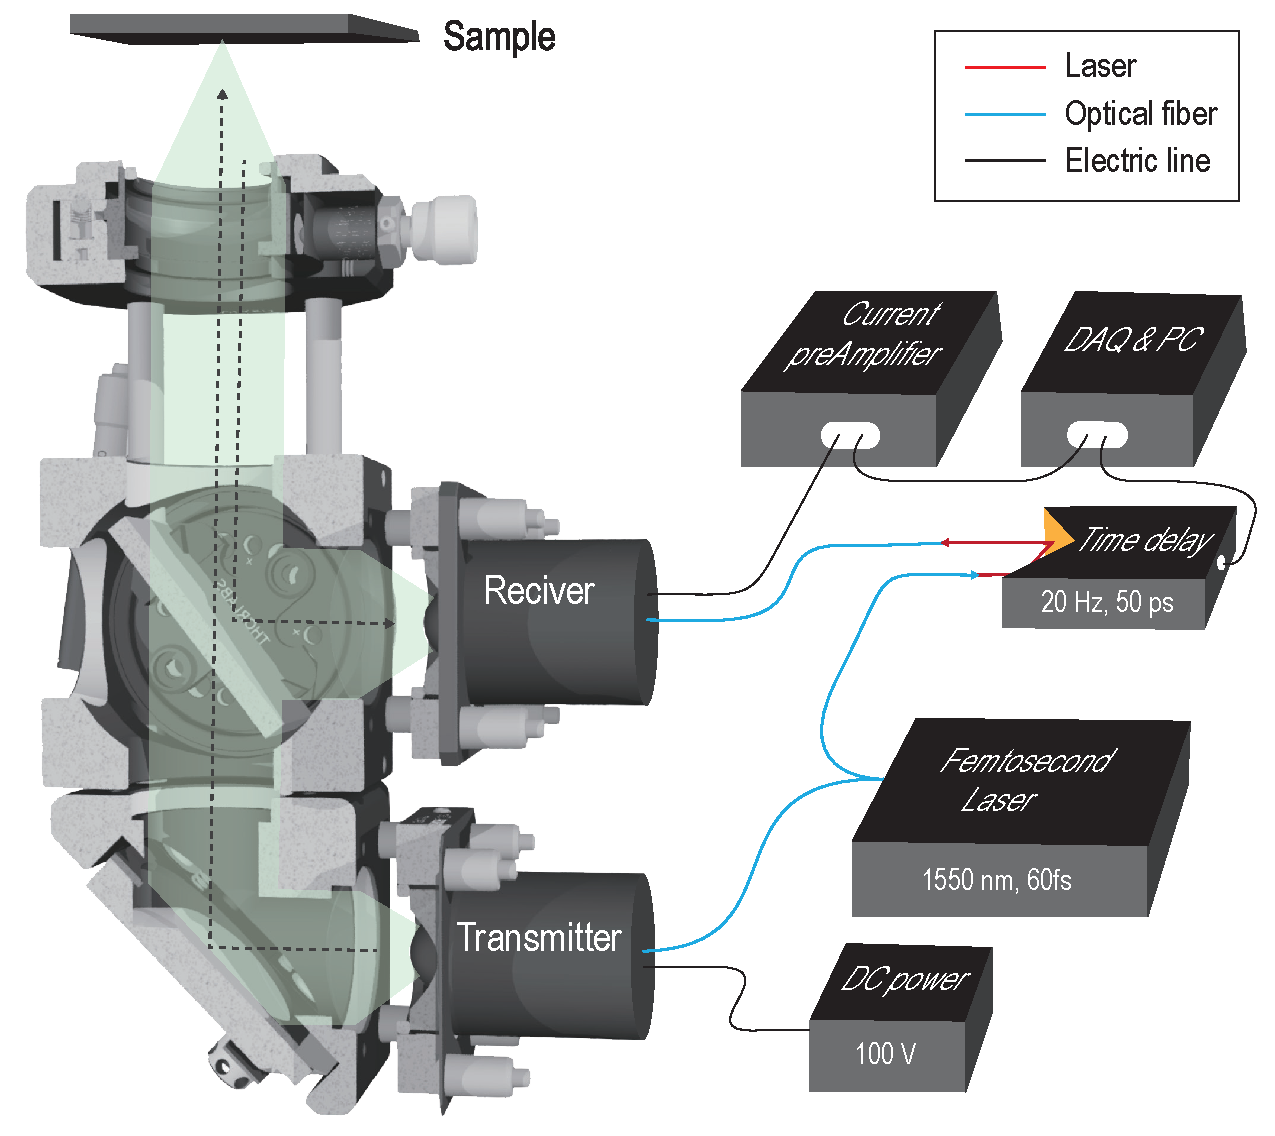
\includegraphics[width=\columnwidth]{fig/Ryu-fig3.pdf}
    \caption{Configuration of a THz-TDS imaging system.}
    \label{fig:system}
\end{figure}


\subsection{Diffraction Limit in Optics} % Preliminary

The diffraction limit refers to the theoretical minimum spatial resolution of optical and electromagnetic imaging systems. Equation~\ref{eq:resolution} expresses the diffraction limit of the system, i.e., the minimum resolvable distance, which is the smallest separation at which two points can be distinguished~\cite{rayleigh1879xxxi,nguyen2017enhancement}. In this equation, $\lambda$ represents the wavelength of light or electromagnetic waves, and $n\sin\theta$ denotes the numerical aperture (NA).

\begin{equation}
\label{eq:resolution}
% R \approx 1.22 \frac{\lambda}{D}
{\displaystyle d={\frac {\lambda }{2n\sin \theta }}={\frac {\lambda }{2\mathrm {NA} }}}
\end{equation}
The NA represents the amount of light or electromagnetic waves that an optical or electromagnetic imaging system can collect from a sample. It is adjustable based on the size of the lens aperture, the distance between the lens and sample, and the refractive index of the medium. However, once the wavelength of the light or electromagnetic waves is determined by the source constituting the imaging system, it cannot be adjusted: thus, the diffraction limit of the system is determined by the wavelength of the source.

As the frequency increases, the wavelength decreases, thus enhancing the spatial resolution of the imaging system (theoretically). However, in typical THz imaging systems, the output of the system decreases as the frequency increases, thus increasing the amount of noise and rendering the acquisition of  high-quality images difficult. Hence, models are trained using THz SAHS images acquired using a THz-TDS system. By applying these models to images obtained at lower frequencies with sufficient output, and performing inferences, one can obtain results similar to those yielded at higher frequencies can be achieved. This method allows enables overcoming the diffraction limit of frequencies in imaging systems. In other words, it allows for surpassing the spatial resolution limits of low-frequency imaging systems with sufficient output, thereby generating images equivalent to those at the diffraction limit of higher frequencies.


\subsection{Overall Framework}
We propose a new mage restoration method that overcomes the diffraction limit through self-supervised learning using THz SAHS images acquired from a THz-TDS reflective system. Fig.~\ref{fig:overall} illustrates the overall framework of the proposed image restoration method. The first stage of this framework involves learning from one frequency image to another, which abbreviated as one-to-one (O2O). The second stage, named recurrent (RE), involves repeating the previous stage by replacing the input with previous target and the target with previous output of the model. The third stage is ZSSR, where the image resolution increases using the image by itself. The stages are described in the corresponding subsections.

\begin{figure}[htbp]
    \centering
    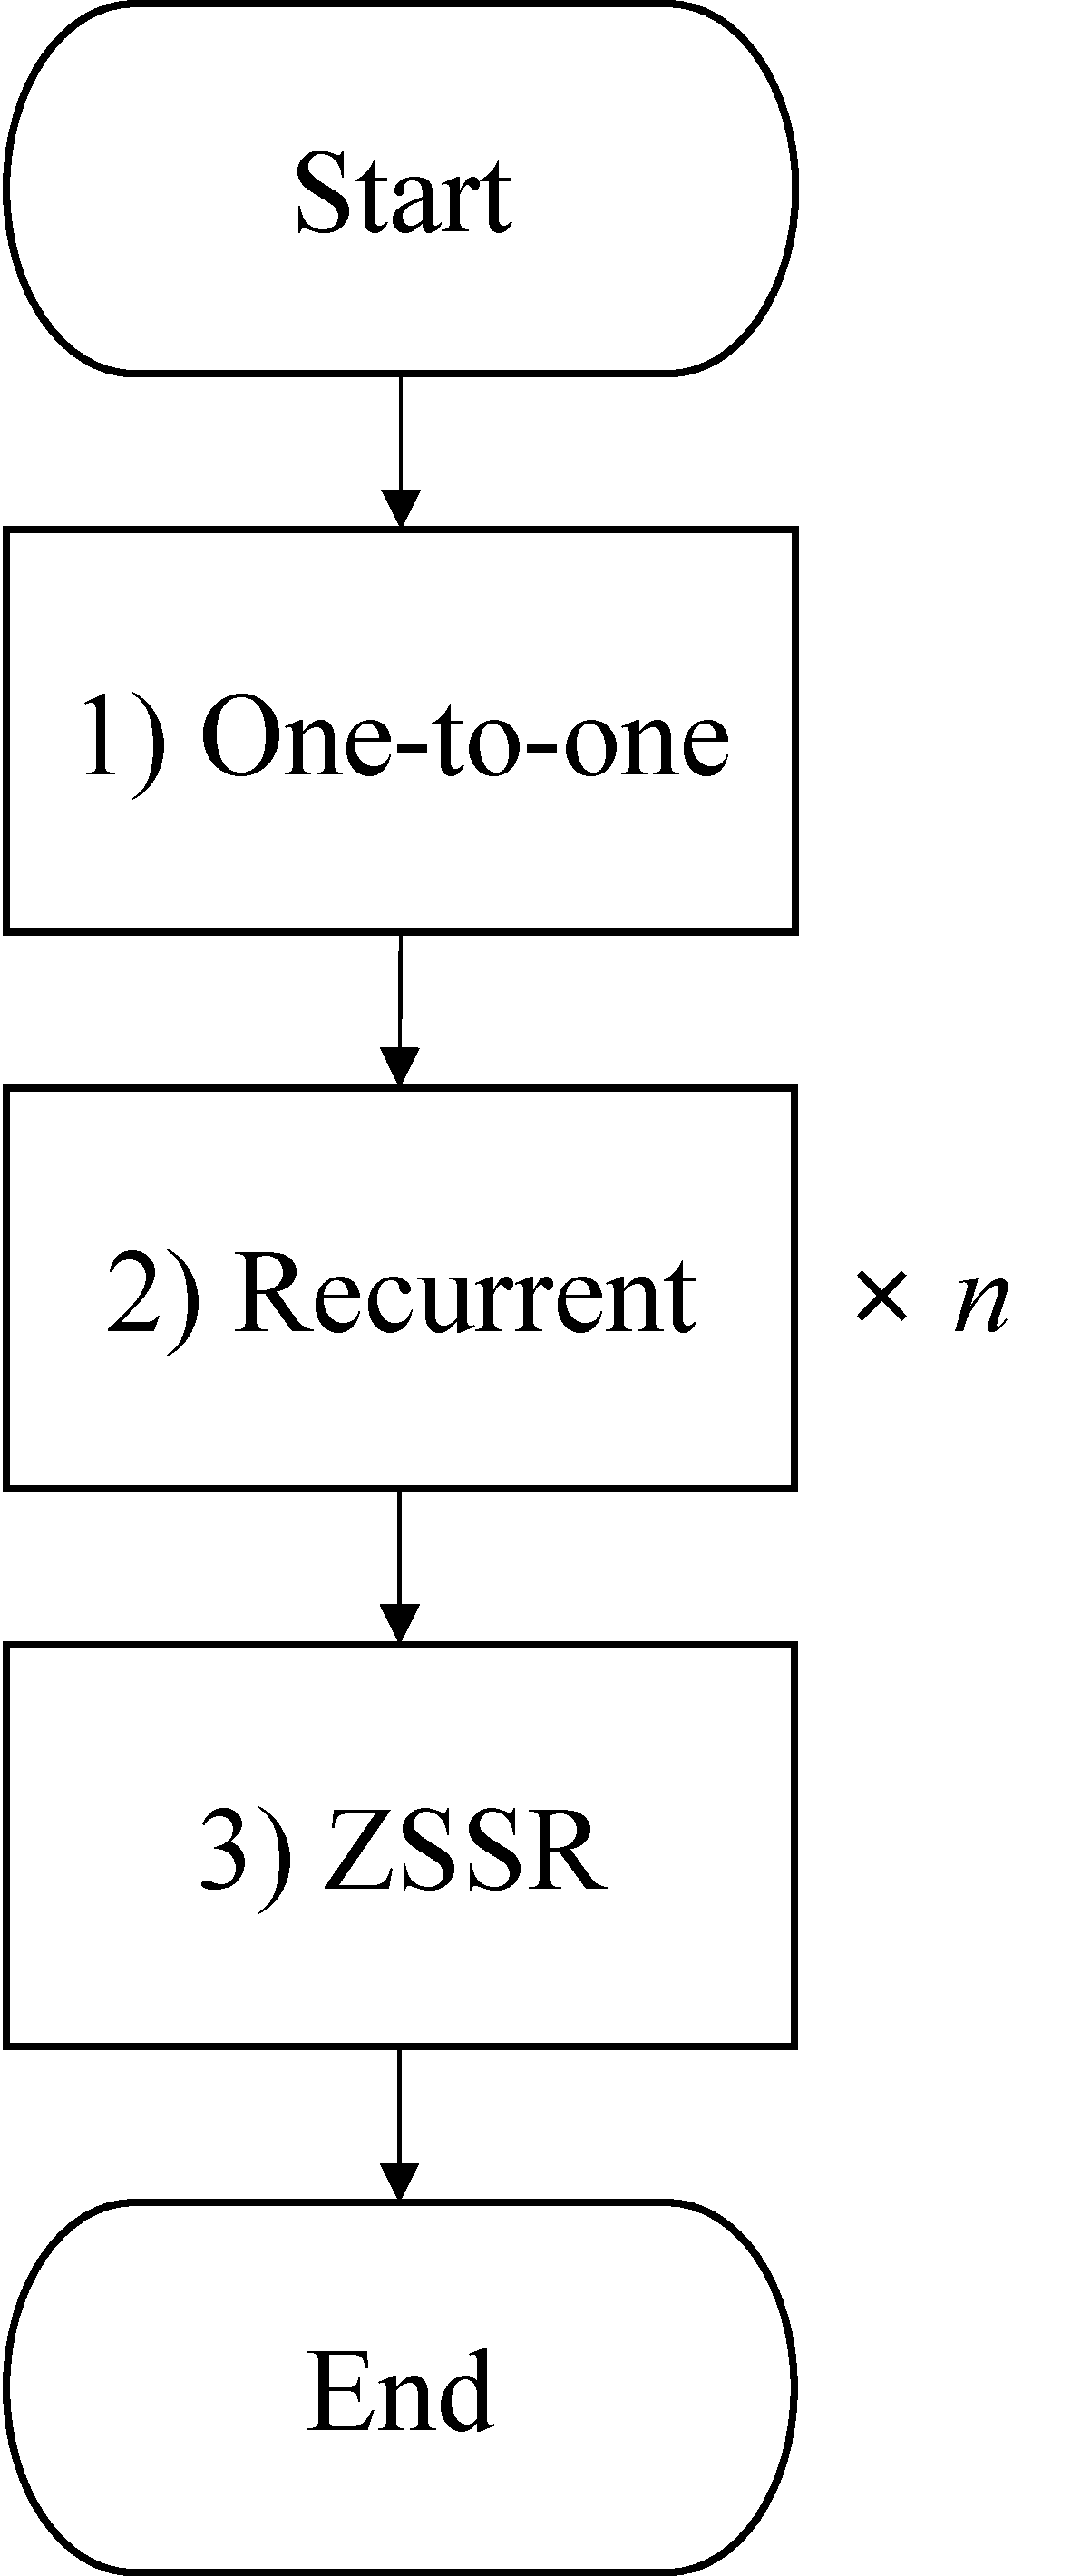
\includegraphics[width=0.3\columnwidth]{fig/Ryu-fig4.pdf}
    \caption{Overall framework of proposed image restoration method.}
    \label{fig:overall}
\end{figure}

\subsubsection{O2O}
O2O mapping learning is conducted in this study, in which one image is trained to follow the characteristics of another image. This allows the network to be trained such that the low-frequency images can mimic the characteristics of the high-frequency images. In this method, a deep neural network $\mathcal{D}$ with learning parameters $\Theta$ is trained to map an image at $\alpha$ THz, $I_\alpha$, to an image at $\beta$ THz, $I_\beta$. The objective of the training is to obtain the parameter $\Theta$ such that minimizes the loss between the output image $\mathcal{D}({I_\alpha};\Theta)$ generated through the network and target image $I_\beta$, as expressed in Equation~\ref{eq1}.

\begin{equation}
\argmin_{\Theta} \mathcal{L}(\mathcal{D}({I_\alpha};\Theta), I_\beta),
\label{eq1}
\end{equation}
where $\mathcal{L}$ denotes the loss function for supervised learning.

In this study, the network is trained using source images, with target images serving as the ground truth. During the inference, the input images used are called inference images. A network trained with $I_\alpha$ as the source and $I_\beta$ as the target is succinctly denoted as $\mathcal{D}_{I_\alpha\rightarrow I_\beta}$. The process of inferring an image at $\gamma$ THz, $I_\gamma$, using this model can be written as
\begin{equation}
\mathcal{D}_{I_\alpha\rightarrow I_\beta}(I_\gamma).
\end{equation}

Fig.~\ref{fig:o2o_explain} illustrates the training and inference procedures of the One-to-one method. Fig.~\ref{fig:o2o_explain}(a) shows the training process. As described earlier, based on $I_\alpha$ as the source and $I_\beta$ as the target, the network is trained to minimize the loss between the network output and target. Fig.~\ref{fig:o2o_explain}(b) shows the process of inferring an inference image $I_\gamma$, obtained within (intra) the THz SAHS images, using the trained network $\mathcal{D}_{I\alpha\rightarrow I_\beta}$, which is termed ``intra-data inference.'' As shown in Fig.~\ref{fig:o2o_explain}(c), the same network is used for cross-data inference, where a new image $J$, which is unrelated to the THz SAHS images used for training, is inferred. Image $J$ can exhibit a completely different form the training images and can be obtained using a system different from that used for the training images. This process is known to as ``cross-data inference.''

\begin{figure*}[htbp]
    \centering
    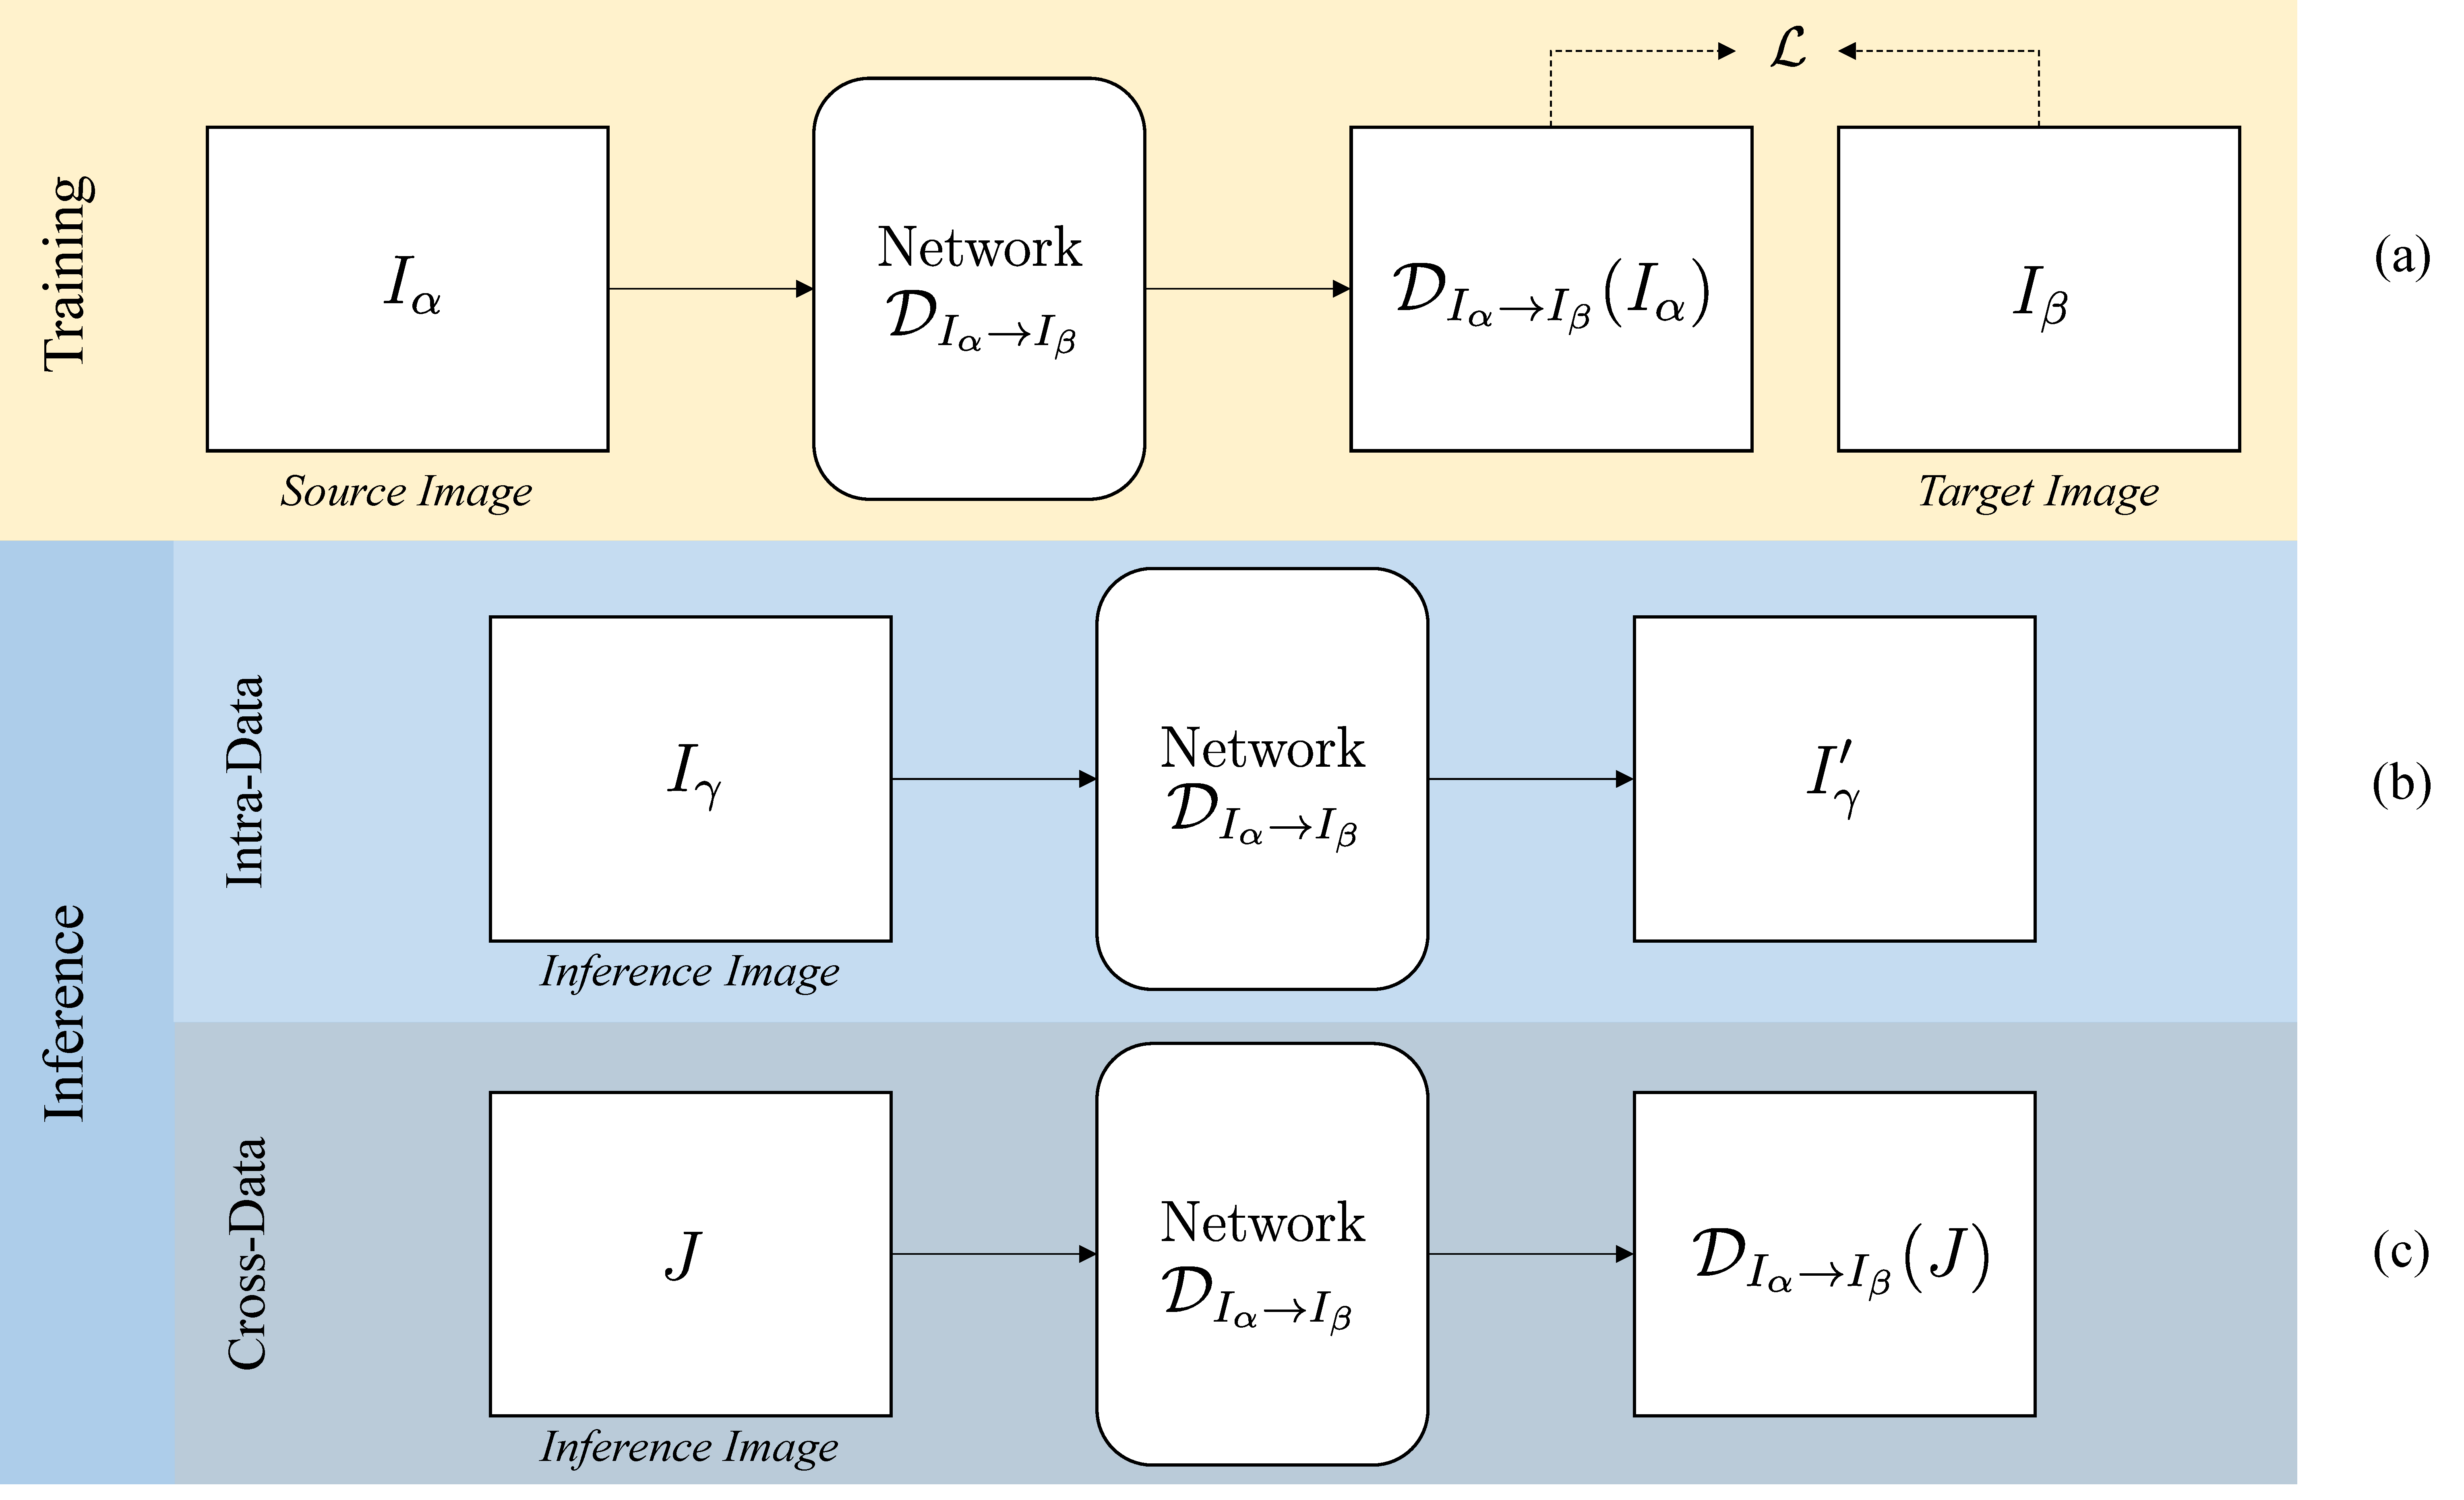
\includegraphics[width=0.7\textwidth]{fig/Ryu-fig5.pdf}
    \caption{O2O training and inference process. (a) Training; (b) inference with intra-data; (c) inference with cross-data.}
    \label{fig:o2o_explain}
\end{figure*}

The results of applying $I_\gamma$ vary depending on how $\alpha$ and $\beta$ are set. Using a model that maps from low to high frequency $(\alpha < \beta)$ enhances the spatial resolution of low-frequency images. This enhancement occurs because the blurry low-frequency images mimic the sharpness of the high-frequency images, thereby overcoming the diffraction limit of the low-frequency images. Conversely, mapping an image obtained from high-frequency with a weak signal in the THz-TDS system to an image obtained from low-frequency with a relatively stronger signal  $(\alpha > \beta)$ helps in reducing noise in high-frequency images, although this may introduce some blurring owing to the emulation of low-frequency images. The model trained as such can be applied to new THz images unrelated to the training data to enhance image sharpness or reduce noise. More detailed experimental results are presented in Section~\ref{sec:exp}.

\subsubsection{RE}
The image inferred using a network trained using the One-to-one method is used as a target for repeating the O2O training. This process, which is repeated $n$ times, allows for further improvements to the enhanced image and is abbreviated as RE.

After conducting One-to-one training, the result of inferring $I_\beta$ using the obtained model is denoted as $I_\beta'$. This can be expressed as shown in Equation~\ref{eq:o2o}.
\begin{equation}
\mathcal{D}_{I_\alpha\rightarrow I_\beta}(I_\beta) = I_\beta'.
\label{eq:o2o}
\end{equation}

Subsequently, it is used as a target and $I_\beta$ is used as a source for further training; next the model is used to infer $I_\beta'$. This result is denoted as $I_\beta''$, which can be expressed as shown in Equation~\ref{eq:re1}.
\begin{equation}
        \mathcal{D}_{I_\beta\rightarrow I_\beta'}(I_\beta') = I_\beta''.
        \label{eq:re1}
\end{equation}
This process can be repeated recurrently. However, as will be discussed in Section~\ref{sec:exp}, excessive repetition of this process can yield unnatural visual results. The result of performing RE twice can be expressed as shown in Equation~\ref{eq:re2}.
\begin{equation}
    \mathcal{D}_{I_\beta'\rightarrow I_\beta''}(I_\beta'') = I_\beta'''.
    \label{eq:re2}
\end{equation}

\begin{figure*}[htbp]
    \centering
    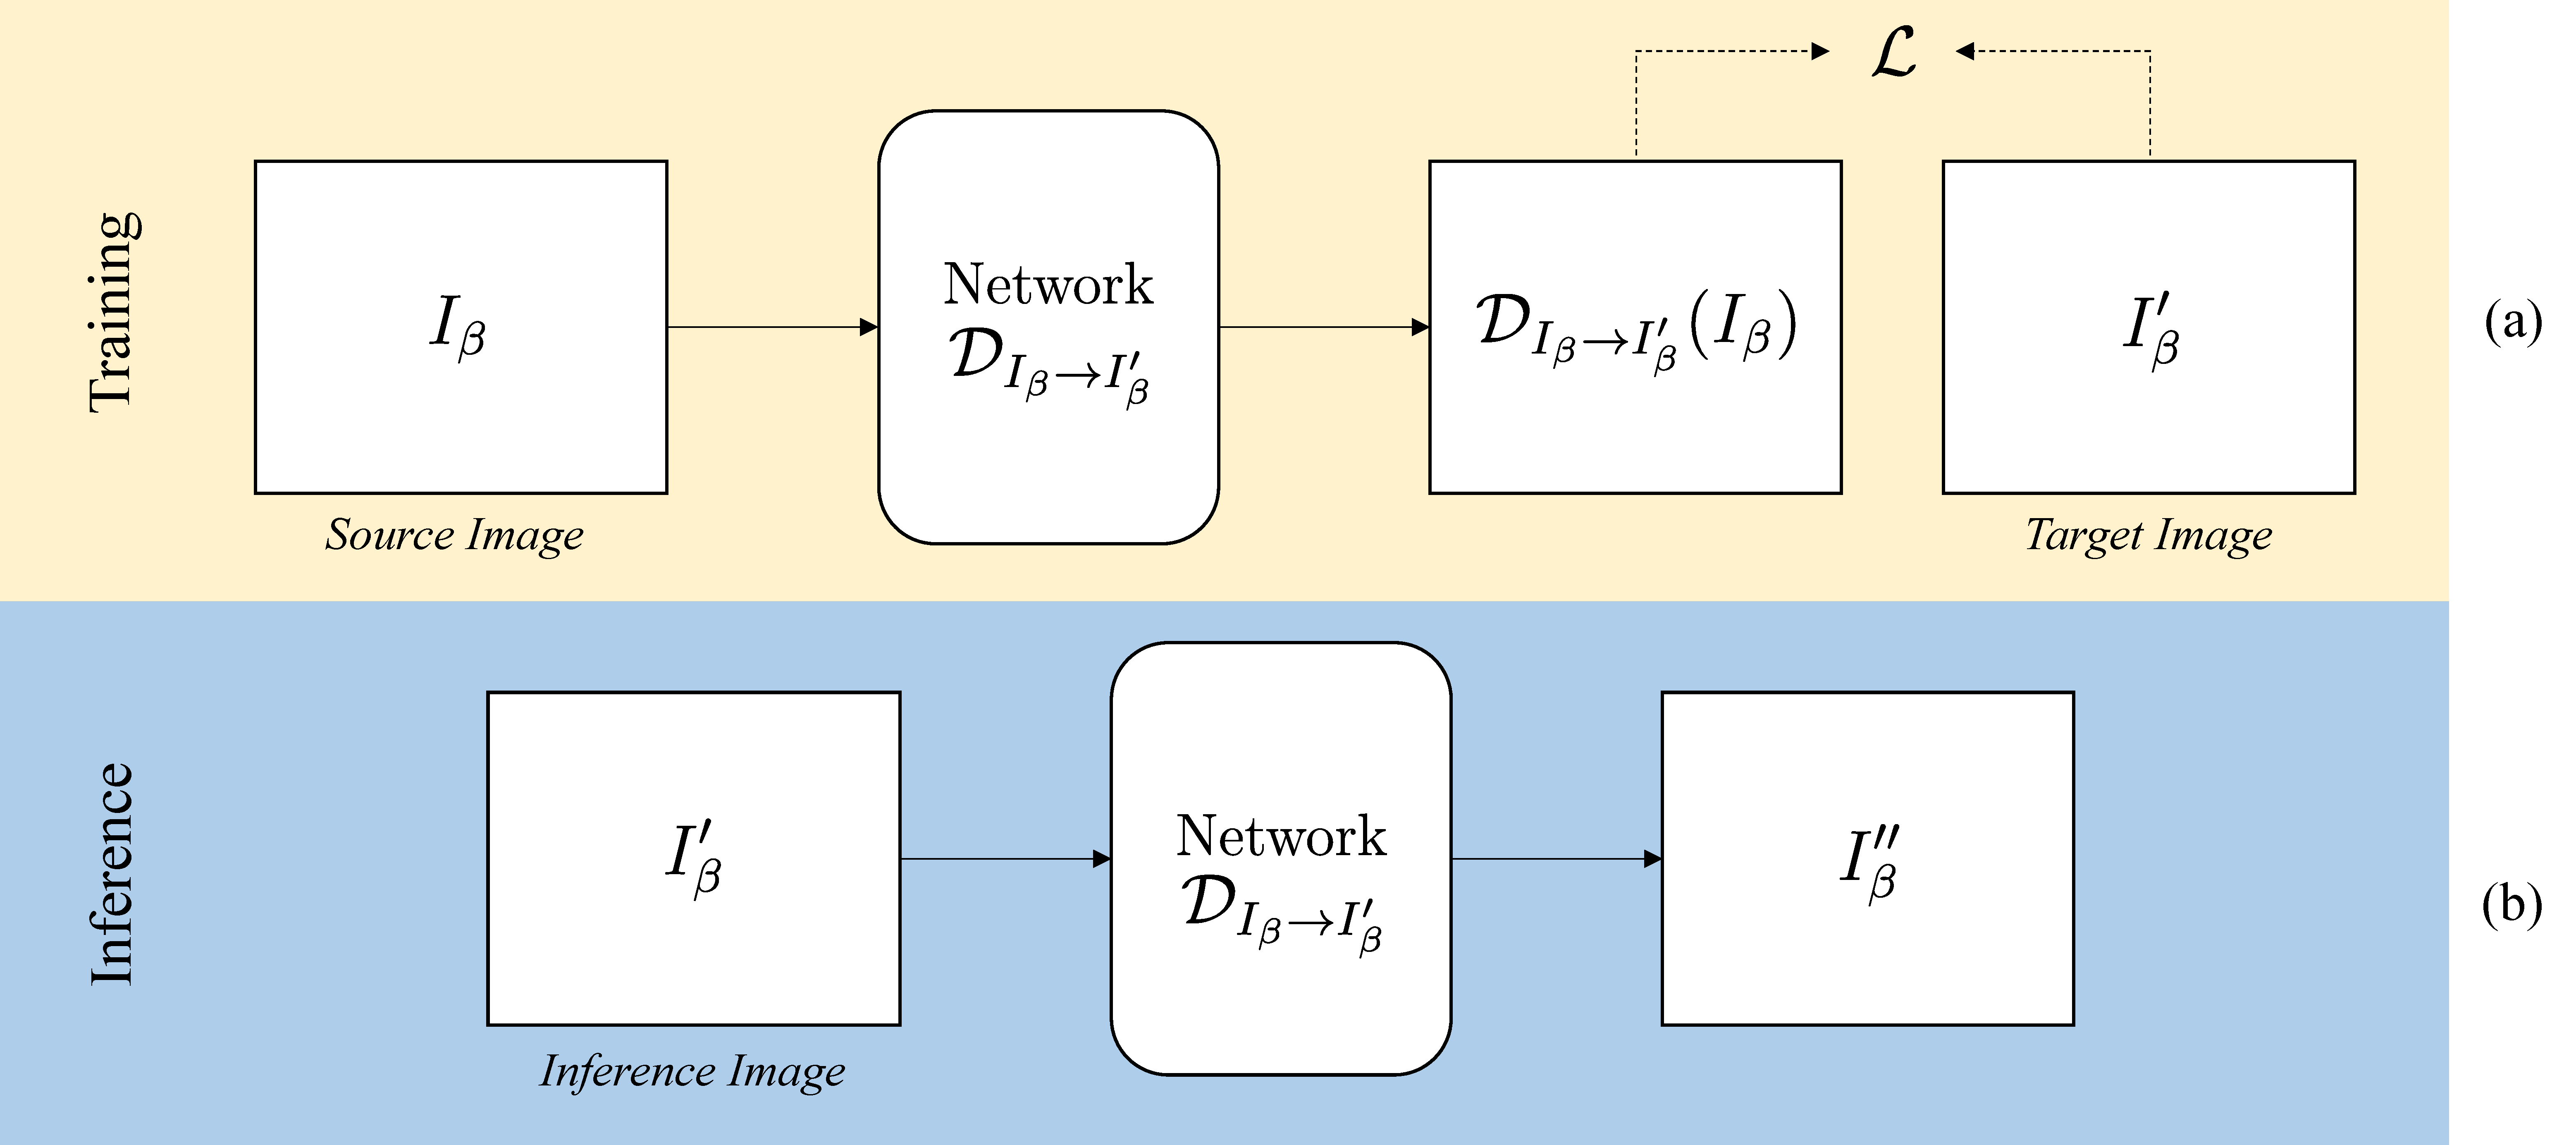
\includegraphics[width=0.7\textwidth]{fig/Ryu-fig6.pdf}
    \caption{RE training and inference process. (a) Training; (b) inference.}
    \label{fig:recurrent_explain}
\end{figure*}
Fig.~\ref{fig:recurrent_explain} shows the training and inference processes of the RE method. It involves the same procedure as O2O; however, the source and target images used are the target and inference results of O2O, respectively.


\subsubsection{ZSSR}
ZSSR is an unsupervised image SR method proposed in~\cite{shocher2018zssr}. Unlike traditional super-resolution methods, ZSSR operates without the need for pre-training on large external datasets. Instead, this method identifies patterns and structures repeated within a single input image and uses these findings as a basis to learn SR transformations. During inference, the model is dynamically trained, allowing the learned model to be immediately used to infer a high-resolution version of the input image. It can adapt to different image settings, thus enabling SR on old photographs, noisy images, biological data, and other images with unknown or non-ideal acquisition processes. The ability of this method to train on a single image renders it particularly suitable for THz images, in which accurately estimating blur and noise is challenging. In addition, because of the general difficulty in obtaining high-resolution THz images, applying ZSSR can yield the best quality images under the resources of the THz imaging system in use. Fig.~\ref{fig:zssr_explain} shows the training and inference processes involved in the ZSSR technique. The inference image $I$, initially downscaled by a scale factor $s$, is then used as the source, with $I$ as the target, to train the SR network. After training, the SR network's weights are used to infer $I$, thus resulting in an image with width and height increase by a factor of $s$.

\begin{figure*}[htbp]
    \centering
    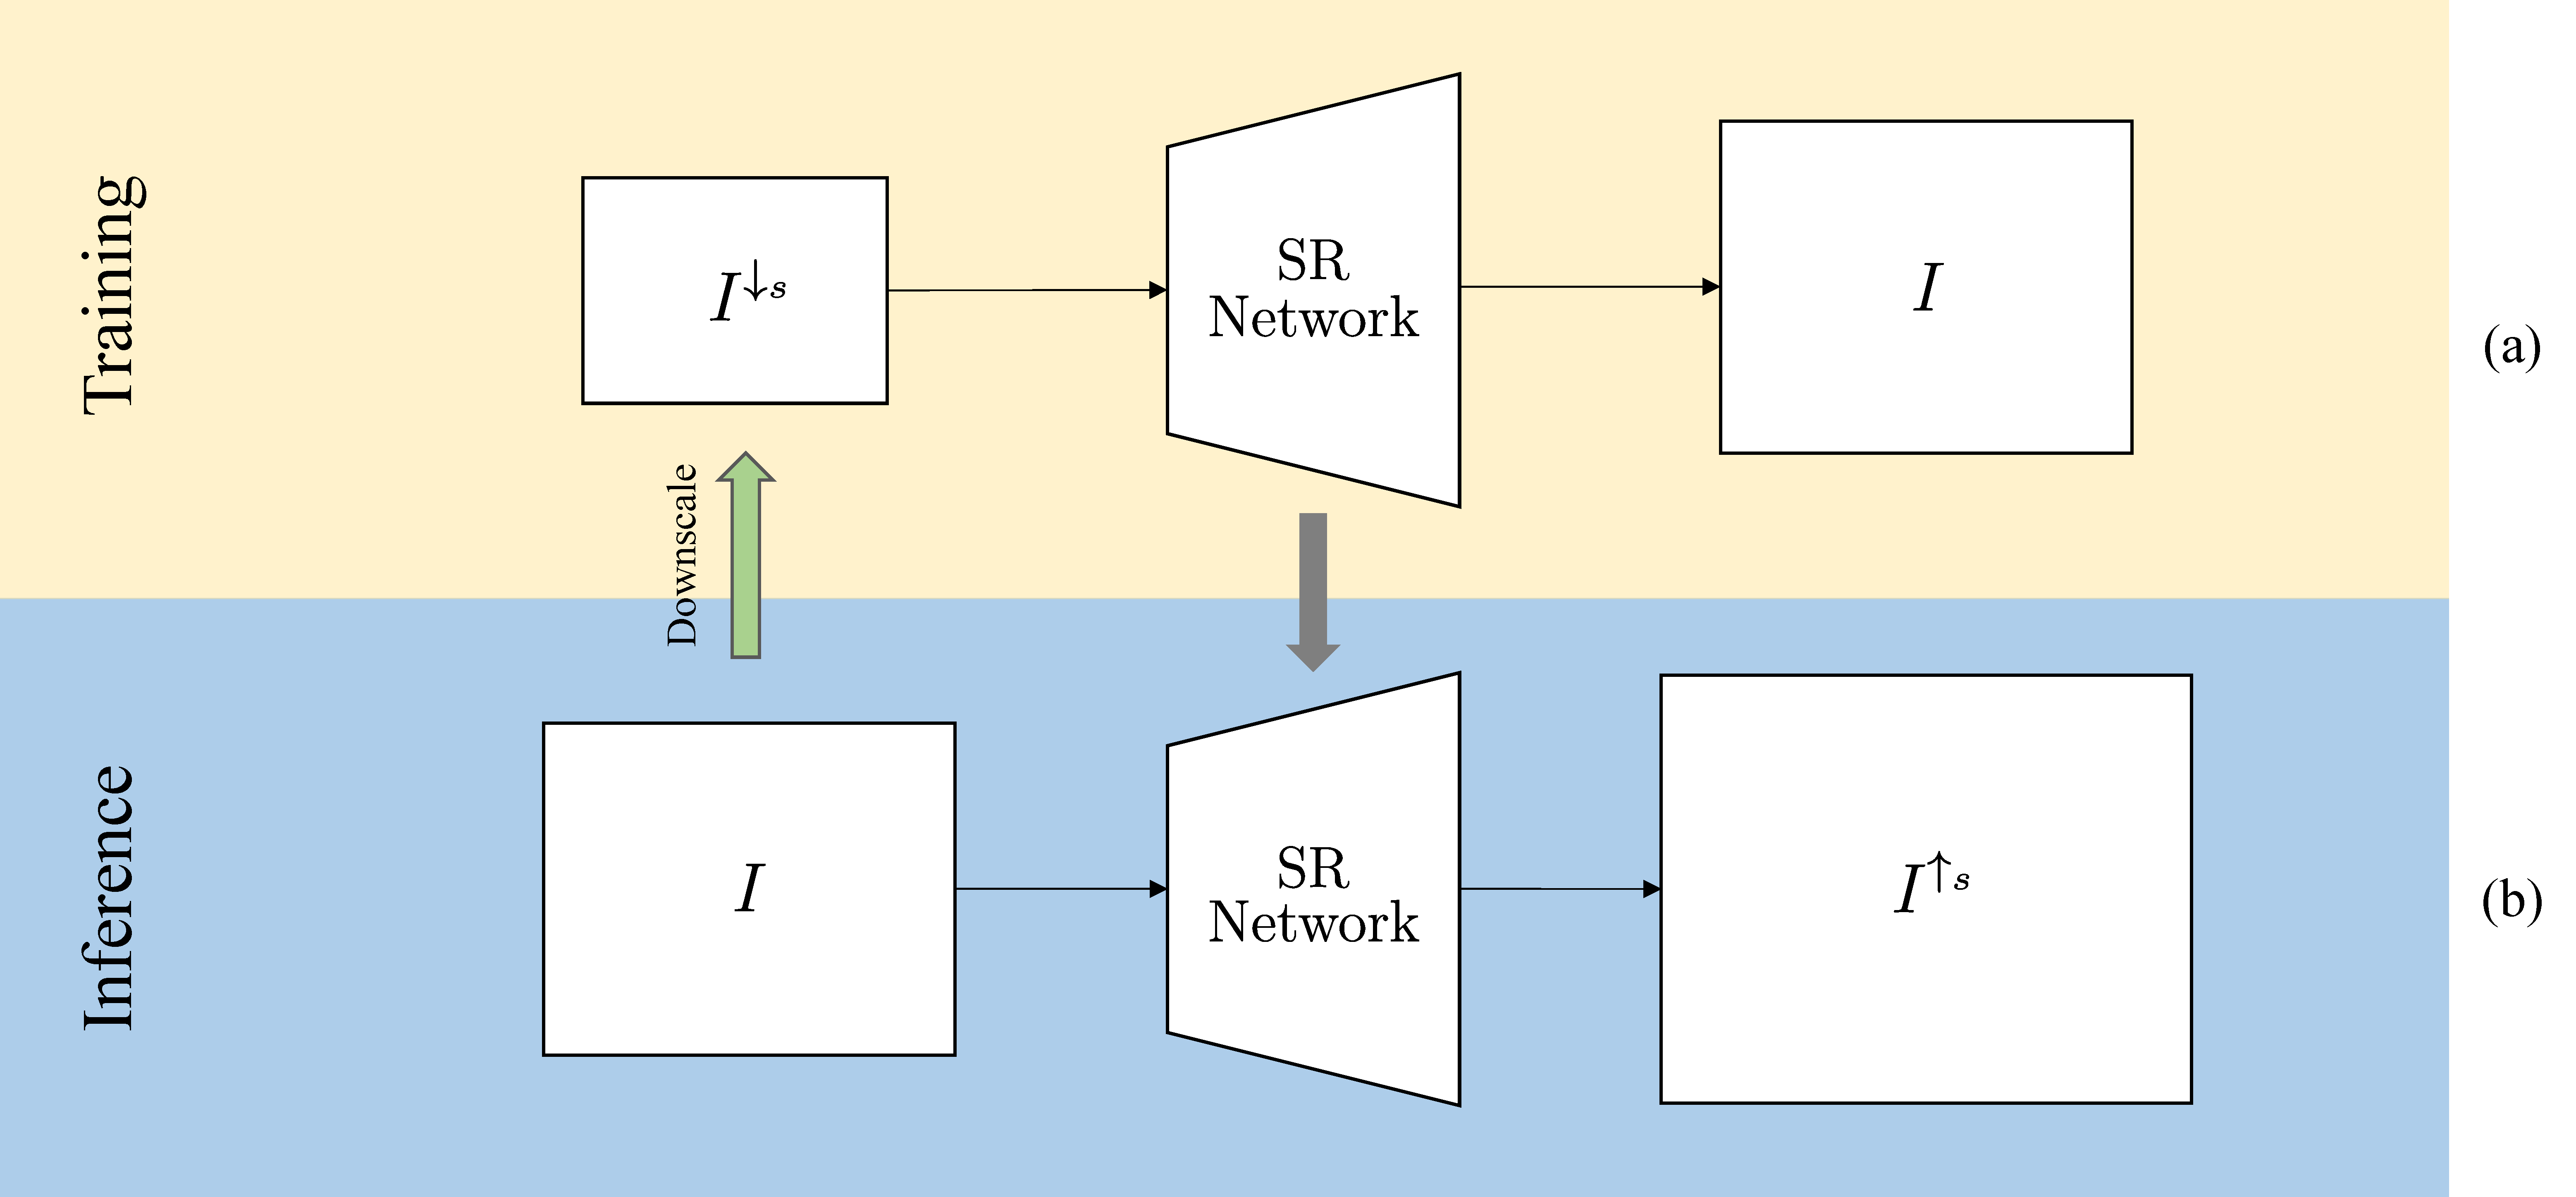
\includegraphics[width=0.65\textwidth]{fig/Ryu-fig7.pdf}
    \caption{ZSSR training and inference process. (a) Training; (b) inference.}
    \label{fig:zssr_explain}
\end{figure*}